\documentclass[12pt,a4paper]{memoir}
%\usepackage[utf8]{inputenc}
% \usepackage[T1]{fontenc}

%%
%% LDA video lecture https://www.youtube.com/watch?v=DDq3OVp9dNA
%%
% \usepackage{microtype}
\usepackage[dvips,xetex]{graphicx}
% \usepackage{xcolor}
\usepackage{amsmath}
\usepackage{lipsum}
\usepackage{breakcites}
\usepackage{rotating}
% \usepackage{times}

\usepackage{algorithm}
\usepackage{algpseudocode}% http://ctan.org/pkg/algorithmicx
\usepackage{tikz}
\usepackage{booktabs}
% \usepackage{caption}
% \usetikzlibrary{matrix,shapes,arrows,positioning,chains}
\usetikzlibrary{shapes.geometric, arrows}
% \usepackage[LGRgreek]{mathastext}
% incompatible \usepackage{cite}
% \usepackage[sorting=none, 
% style=verbose, citestyle=alphabetic
% ]{biblatex}
\usepackage{algorithmicx}
\usepackage{float}
\usepackage{setspace}
%\bibliography{MyCollection}
% \addbibresource{MyCollection.bib} %Imports bibliography file
% \usepackage{blindtext}
\usepackage{ragged2e}

% \usepackage{emptypage}

%% \renewcommand{\nomname}{List of Symbols}
%%%% list of symbols package below

\usepackage[symbols,nogroupskip,sort=none]{glossaries-extra}

\glsxtrnewsymbol[description={alpha}]{a}{\ensuremath{\alpha}}
\glsxtrnewsymbol[description={velocity}]{v}{\ensuremath{\epsilon}}
\glsxtrnewsymbol[description={Rating of $i_{th}$ User}]{ri}{\ensuremath{R_i}}
\glsxtrnewsymbol[description={Dirichlet Distribution}]{lda}{\ensuremath{\Phi}}

% \usepackage{textcomp}
%% for the font     \usepackage{mathptmx}
% \usepackage[Rejne]{fncychap}
% Sonny, Lenny, Glenn, Conny, Rejne, Bjarne, Bjornstrup

\usepackage[
breaklinks=true,colorlinks=true,
% linkcolor=blue,urlcolor=blue,citecolor=blue,anchorcolor=blue,% PDF VIEW
linkcolor=black,urlcolor=black,citecolor=black,% PRINT
bookmarks=true,bookmarksopenlevel=2]{hyperref}

\usepackage{geometry}
% PDF VIEW
% \geometry{total={210mm,297mm},
% left=30mm,right=25mm,
% bindingoffset=0mm, top=30mm,bottom=25mm}
% PRINT
\geometry{left=30mm,
right=25mm,
top=30mm,
bottom=25mm,
heightrounded,}

%\OnehalfSpacing
\linespread{1.3}

%% Custom Chapter Style
% \usepackage{calc,fourier}
\usepackage{calc}
\makeatletter
\setlength\midchapskip{7pt}
\makechapterstyle{VZ21}{
    \renewcommand\chapnamefont{\Large\scshape}\renewcommand\chapnumfont{\Large\scshape\centering}\renewcommand\chaptitlefont{\huge\bfseries\centering}\renewcommand\printchaptertitle[1]{
        \setlength\tabcolsep{7pt}% used as indentation on both sides
        \settowidth\@tempdimc{\chaptitlefont ##1}%
        \setlength\@tempdimc{\textwidth-\@tempdimc-2\tabcolsep}
        \chaptitlefont
        \ifdim\@tempdimc > 0pt\relax% one line
        \begin{tabular}{c}
            \toprule  ##1\\ \bottomrule
        \end{tabular}
        \else% two+ lines
        \begin{tabular}{%
            >{\chaptitlefont\arraybackslash}p{\textwidth-2\tabcolsep}}
            \toprule ##1\\ \bottomrule
        \end{tabular}
        \fi
    }
}
\makeatother

%%% CHAPTER'S STYLE
% \chapterstyle{bianchi}
% \chapterstyle{ger}
% \chapterstyle{madsen}
% \chapterstyle{ell}
% \chapterstyle{companion}
% \chapterstyle{hansen}
% \chapterstyle{verly}
% \chapterstyle{crosshead}
% \chapterstyle{veelo}
% \chapterstyle{thatcher}
% \chapterstyle{southall}
\chapterstyle{VZ21}
% \chapterstyle{VZ23}
% \chapterstyle{VZ34}
% \chapterstyle{VZ43}
%%% STYLE OF SECTIONS, SUBSECTIONS, AND SUBSUBSECTIONS
\setsecheadstyle{\Large\bfseries\sffamily\raggedright}
\setsubsecheadstyle{\large\bfseries\sffamily\raggedright}
\setsubsubsecheadstyle{\bfseries\sffamily\raggedright}


%%% STYLE OF PAGES NUMBERING
%\pagestyle{companion}\nouppercaseheads 
%\pagestyle{headings}
%\pagestyle{Ruled}
\pagestyle{plain}
\makepagestyle{plain}
\makeevenfoot{plain}{\thepage}{}{}
\makeoddfoot{plain}{}{}{\thepage}
\makeevenhead{plain}{}{}{}
\makeoddhead{plain}{}{}{}


\maxsecnumdepth{subsection} % chapters, sections, and subsections are numbered
\maxtocdepth{section} % chapters, sections, and subsections are in the Table of Contents
\renewcommand{\baselinestretch}{1.3}

%%%---%%%---%%%---%%%---%%%---%%%---%%%---%%%---%%%---%%%---%%%---%%%---%%%

\begin{document}
%%%---%%%---%%%---%%%---%%%---%%%---%%%---%%%---%%%---%%%---%%%---%%%---%%%
%   TITLEPAGE
%
%   due to variety of titlepage schemes it is probably better to make titlepage manually
%
%%%---%%%---%%%---%%%---%%%---%%%---%%%---%%%---%%%---%%%---%%%---%%%---%%%

\stepcounter{section}
\thispagestyle{empty}
%\vspace*{1.0cm}
{\centering
    {{A Thesis of}\\}
    %       \vspace{0.1cm}
    %       \vspace{0.1cm}
    \vspace{0.1cm}
    {\Large\textbf{Modeling Product Ratings and Reviews using Latent Factors to provide Recommendations}\\}
    \vspace{1cm}
    {\textit{Submitted in partial fulfillment of the requirements for the degree of}\\}
    \vspace{0.5cm}
    {\textbf{Master of Technology}}
    \\\textit{in}
    \\{\textbf{Computer Science and Engineering}}
    \vspace{1cm}
    \\{\textit{by}}\\
    \vspace{0.2cm}
    {\large \textbf{Rahul Bali}} \\ (Roll No. 16205025)\\
    \vspace{1.5cm}
    % {\textit{under the supervision of}} \\
    % \vspace{0.2cm}
    % { Prof. Shilpa Verma }\\
    \vspace {0.7cm}
    \begin{figure}[h]
        {\centering {
\includegraphics[width = .40 \textwidth]{logo.jpg}}\par}
    \end{figure}
    \vspace{0.5cm}
    {\normalsize{\textbf{DEPARTMENT OF COMPUTER SCIENCE AND ENGINEERING}}}\\
    \vspace{0.3cm}
    {\textbf{PUNJAB ENGINEERING COLLEGE\\}}
    {\textbf{CHANDIGARH, INDIA\\}}
    \vspace{.2 cm}
    {JUNE 2018}\\
}
%\pagebreak

\cleardoublepage
%%%---%%%---%%%---%%%---%%%---%%%---%%%---%%%---%%%---%%%---%%%---%%%---%%%
%%%---%%%---%%%---%%%---%%%---%%%---%%%---%%%---%%%---%%%---%%%---%%%---%%%


%\sfdefault
\frontmatter % make the front page numbers roman

\section*{Acknowledgement}
\addcontentsline{toc}{chapter}{Acknowledgement}
It is always a pleasure to finish a research project on a high note. It gives extra pleasure while looking back working with kind, humble and wise people. 

First of all, I would like to thank the Almighty God for helping me to successfully finish this project. Her blessings guided me through some of the hard times in my life and showed me the correct path. I would like to express my heartfelt gratitude to my supervisor Prof. Shilpa Verma for allowing me to work with her, helping me to see it through to completion. She was very supportive, encouraging, patient during the whole life-cycle of the project and the final thesis preparation. She took the pain of reading through the initial drafts of my thesis during her busy schedule and I am greatly thankful to her for the suggestions regarding the structure and content of final paper. I thank my examiner for reading through the final paper and making the necessary arrangements for the successful presentation.

Finally, I would like to thank my family, colleagues and friends, for all the support given during the project implementation stage.\\\\\\\\

\begin{minipage}{0.4\textwidth}
-
\end{minipage}% don't leave space after this
\begin{minipage}{0.6\textwidth}
\textbf{Rahul Bali} 16205025\\
M.Tech, Computer Science and Engineering\\
Punjab Engineering College\\
Chandigarh - 160012, India\\
Phone: +91-8901337758\\
Email: rahulrdb18@gmail.com 
\end{minipage}


\clearpage
\listoffigures

\clearpage
\listoftables

%%%%%%%%%%%%%%%%%%%%%%%%

% \printunsrtglossary[type=symbols,style=long,title={List of Symbols}]

% \chapter{Sample}
% Reference symbols: $\gls{x}$, $\gls{v}$, $\gls{a}$, $\gls{t}$,
% $\gls{F}$.

\cleardoublepage

\tableofcontents*


%%%%%%%%%%%%%%%

\clearpage

%%%---%%%---%%%---%%%---%%%---%%%---%%%---%%%---%%%---%%%---%%%---%%%---%%%
%%%---%%%---%%%---%%%---%%%---%%%---%%%---%%%---%%%---%%%---%%%---%%%---%%%

%\centering
\begin{center}
\normalsize\textbf{Abstract}\\
\justify
The world has seen many recommender systems online or offline. More or less the working is the same for both. In recommender systems, item-based collborative filtering is a
\end{center}



\cleardoublepage

\mainmatter % normal page numbers start here
\chapter{Introduction}

\section{Background}

Recommender Systems is a hot topic within Computer Science, as algorithms for the purpose of targeted advertisement get improved each year. Hence it is vital for companies to keep up with their competitors. Personal integrity, or online privacy, is also a frequently discussed topic within computer science, as well as, in society and on a global level. How much and what kind of data is ethically acceptable to observe in order to produce relevant advertisements? Is it acceptable to use all data that could be retrieved
from a user such as GPS-based movement, cookies, chat-history, previous purchases or other arbitrary personal data a company might have access to?

This thesis focuses on the evaluation and analysis of the performance of "Item-based Collaborative filtering" for the purpose of targeted advertisement within e-commerce.

---- make changes...

Comparisons are made with more standard algorithms, being used in many live recommender systems for e-commerce as of today. Whereas the algorithmic approach of Contextual Multi-Armed Bandit algorithms have use-areas within recommender systems, very little research has been made for use within e-commerce. Performance will also be analysed and evaluated taking into consideration how much personal data are observed. How much and what kind of data can be observed and manipulated for it to still be considered socially and ethically acceptable? That is while still respecting the users’ privacy. There exist research on the subject, addressing the issue of online privacy.

\cite{park2012literature}

\section{Methodology}

\section{Related Work}

\section{Scope}

Scope of the dataset explained---

The scope of the dataset intended to be used in this project consists complete database from the Amazon.com - the ecommerce website system from May 1996 - July 2014. We have decided to limit the database to the Digital Music Category only, as the database is sufficient for the experiment. The database also has very contextaul user data and the metadata about the product. This dataset does not contain any sort of the session based data, like click, heat zones, etc.

Amazon Review Dataset contains information about 279,899 products with 836,006 reviews from the Digital Music Category.
The avern   


\begin{verbatim}
       X                asin           helpful          overall    
Min.   :     0   B004D1GZ2E:  1953   [0, 0] :550515   Min.   :1.00  
1st Qu.:209001   B0026P3G12:  1926   [1, 1] : 74079   1st Qu.:4.00  
Median :418002   B0000AGWEC:  1823   [2, 2] : 26928   Median :5.00  
Mean   :418002   B004K4AUZW:  1527   [0, 1] : 25300   Mean   :4.54  
3rd Qu.:627004   B000BGR18W:  1386   [1, 2] : 16855   3rd Qu.:5.00  
Max.   :836005   B00008H2LB:  1325   [3, 3] : 13226   Max.   :5.00  
\end{verbatim}





The scope of the dataset intended to be used in this project consists in the complete
Junkyard database, used live in their e-commerce system from 2009 to 2014. We decided
to limit the project to using only this, as it contains enough sufficient data. The Junk-
yard dataset is very contextual. There is a huge amount of data about each user and all
of their purchases. The Junkyard dataset however has no data regarding click-sessions
from ads or products.
Moreover, the Junkyard dataset initially contains information about several million users
where the average number of orders made by each user is 3.52 and the average number
of items purchased with each order being 2.24.





\section*{Problem Statement}
Amazon uses the most prominent Recommender systems till date for their world class website. The website recommends and portrays the ways for its users to interact with website and find the best products they have been looking for.

These ways are not usually much clearer at first as seeing the number and diversity of the products on the website to choose from. Recommender system plays a very important role here. It provides the best possible recommendations for the user depending upon various aspects of the interaction of the user with the website. These aspects may include user's private information submitted by user itself to the website, location of the user, past purchases of the user, etc. There are endless possibilities for the recommendations to happen on a real world website.

the problem for the semesters the world of 






\chapter{Recommender System}
Recommender system is and remains a hot topic within computer science in 2015. Huge conferences are hosted in different parts of the world annually, featuring many big companies. The RecSys conference [33] is a good example
of this. Recommender Systems has a wide use-area within all kinds of advertisement on the web when specifically targeted ads are needed. These ads can be seen everywhere from websites and apps to emails, text-messages etc. In the list of big actors on the stage of recommender systems, hardly surprisingly, one find companies such as Facebook, Google etc. But Recommender Systems are also used for recommending music in for instance Spotify and movies/TV-shows in Netflix. There are a variety of different algorithms for each use-area. The setting of which this thesis will focus consists
in algorithms for recommender systems within garment-based e-commerce. Here follows some of the more common general techniques used in recommender systems.


\section{Collaborative Filtering}
The basic idea of collaborative filtering is to find information or patterns using collaborative techniques among multiple data sources. Data sources typically consist of users and items such as movies, songs etc. Within e-commerce, and this project specifically, those data sources mainly consist of users, and products that can be bought by these users. Finding these patterns is accomplished through collecting and analysing huge amounts of data on users’ behaviours and activities as well as items. Within e-commerce those activities and behaviours include but are not limited to purchases and click-able ad- vertisements. Collaborative filtering[18] is one of the most common general methods for recommender systems being applicable within several big use-areas. Collaborative Filtering is frequently used in social networks such as Facebook, LinkedIn, mySpace, Twitter etc to effectively recommend new friends, pages, groups as well as who to follow or what to like. But also applications such as Youtube, Reddit, Netflix etc make use of collaborative filtering. Collaborative filtering is viable in all applications where one can observe connections between a user and their registered friends or followers. But it is also widely used within e-commerce, where Amazon is a good example who popularised algorithms for item-to-item based collaborative filtering [21].

Most Collaborative Filtering techniques can be expressed by the two general steps, Similarity Computation and Prediction Generation, described under 2.2

\subsection{User based collaborative filtering}
The main idea of recommender systems built on user-based collaborative filtering consists in computing the similarity between users’ {u,j} profiles, s u\textsubscript{j} . That is, computing a prediction for the probability of the user u liking a specific item i, consists in computing a rating based on all ratings made by users with similar profiles. All similar profiles contribute to this prediction depending on the similarity factor, s uj [34, 35, 36]. 

Typically this can be reduced to the two general steps. 
1. While observing a user’s actions in a system, look for similar users with equal behaviour- and activity-patterns. 
2. Use the observations from step 1 to compute a prediction for the specified user. 

See 2.2 for more information regarding Similarity Computation and Prediction Genera- tion techniques.

\subsection{Item based collaborative filtering}
The concept of item-based collaborative filtering applies the same idea as its User-based counterpart, but the similarity is computed between items instead of users, and is usually described as "Users who bought this also bought that". 

More generally, taking an item-based approach means looking into the set, I, of items a specific user, u, has rated, using their context to compute the similarity of other items, \{i\textsubscript{0} ,i\textsubscript{1} ,...,i\textsubscript{n} \}, not in I. Their corresponding similarities are computed at the same time as {s i0 ,s i1 ,...,s in }. When these similarities and their corresponding items have been found, a prediction can be computed. [36, 37, 38]. 
This can typically be split into three steps: 
1. Construct a User-Item matrix, M[u][i], giving each index of the matrix a rating, r ui , on an item i performed by a user u. 
2. Compute the similarity, s i\textsubscript{1}, i\textsubscript{2}, of two items i 1 and i 2 by looking at co-rated pairs from different users.
3. Generate predictions based on some prediction method, described under 2.2. Item-based collaborative filtering is a very common approach, often used together with algorithms for matrix factorization.

\subsection{Matrix Factorization}
Matrix factorization is an algebraic operation consisting in factorising a matrix M, meaning finding the matrices M 1 ,M 2 ,...,M 3 such that when they are multiplied, the resulting matrix is M. In collaborative filtering based recommender systems this can be used as a rather simple and very intuitive algorithm for discovering latent features. By constructing a User-Item matrix M, where each index contains a rating r on an item i performed by a user u:



\begin{equation*}
\mathBF{M\textsubscript{k,l}} = \left(
\begin{array}{ccc}
x_1 & x_2 & \ldots & x_3 \\
x_3 & x_4 & \ldots & x_2 \\
\vdots & \vdots & \ddots & re
\end{array} 
\right)
\end{equation*}




\chapter{Latent Factor Topic Modelling}

% \begin{figure}[h]
%    {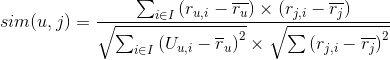
\includegraphics[scale=1]{img/PearsonEqn.png}}
% \end{figure}
Background

However, a number of simple unsupervised methods can also be used for feature selection in text clustering. Some examples of such methods are discussed below.

\section{Document Frequency-based Selection}
The simplest possible method for feature selection in document clustering is that of the use of document frequency to filter out irrelevant features. While the use of inverse document frequencies reduces the importance of such words, this may not alone be sufficient to reduce the noise effects of very frequent words. In other words, words which are too frequent in the corpus can be removed because they are typically common words such as “a”, “an”, “the”, or “of” which are not discriminative from a clustering perspective. Such words are also referred to as stop words.
A variety of methods are commonly available in the literature [76] for stop-word removal.  Typically commonly available stop word lists of
about 300 to 400 words are used for the retrieval process. In addition,
words which occur extremely infrequently can also be removed from
the collection. This is because such words do not add anything to the
similarity computations which are used in most clustering methods. In



3.2



\chapter{Privacy-Preserving Aspects}
Personal integrity is a frequently discussed topic in the connected world.
Most new products today come with the feature of being able to use the Internet; phones, clocks, cars, TVs, baby monitors and even entire households etc.
There are more devices connected to the Internet than there are people living on the planet earth [52]. Being able to stay connected around the clock every day of the month has shed some light on new ethical dilemmas and issues. Internet started out as a place where its users were more or less anonymous. But despite the efforts in present time, creating techniques so as to be more or less anonymous online, a very small portion of the connected world actually make use of these kind of techniques. Applications on our smart devices ask for much more privileges than what their functionality
requires, most of the time. This, however, is the case for most online-based systems in general. People are naive most of the time so as to trust systems and applications with whatever personal information they might ask for. This kind of data can then be sold to companies, authorities or in the worst case, hacked or stolen.

\section{General Aspects of Personal Integrity}
Smart phone applications are a big part of many people's lives. They are used for browsing social medias, calendar and scheduling, public transport, work-out, calorie-tracking, storage, e-commerce and just about anything else. Commonly applications do not ask for any privileges when they are new. However, as the amount of users increase one can be certain that sooner or later the application might ask for extended privileges [53] such as access to files, text-messages, contacts and in some cases even camera and GPS. Most people do not see an issue with this, if it is a good application. In many cases this might not even be a problem. Commonly, regular people, would not complain about an applications performing movie, TV-shows or shopping recommendations despite using all possible private data, as long as the recommendations are valid. In many cases, data changes hands every now and then. Mostly probably because of being sold. What most people do not think of is the fact that once data hits the Internet, it is out of control. Most of the time one can never be sure where its personal data ends up. The more places containing our personal data, the bigger the chance is of it getting leaked, hacked or stolen[54]. These issues are obviously not limited to smart phone applications. It concerns other applications that possess personal information as well. It could be games, e-commerce systems, normal web sites and systems connected to the web in general. It becomes relevant in e-commerce platforms that make use of complex recommender systems and personalised predictions, as those personalised predictions are based on personal information, actions and behaviour in the system. See Chapter 2 for more about recommender systems. To this comes ethical dilemmas; People actively choose to provide companies with their personal data through consistent use of their applications and products. From the aspect of the groups possessing this kind of data, what is ethically acceptable to do with it? Could it be sold or distributed freely? See [55] and [56] for further research on this topic.


There are several techniques, of which most are very easy to use, the regular user can apply to achieve good privacy when browsing the web. Other than common sense such as to be careful and critical, normal methods are through use of proxy servers and virtual private networks. One of the more popular techniques as of last years are through use of onion routing protocols [57]. Onion routing means using layers of encryption where each layer consists of decryption at individual nodes. After decryption is done at each individual node the next destination node, in the chain of nodes, is uncovered. As the message reaches the final destination there should be only one layer of encryption left, which when decrypted provides the original message. Because of each individual node only knowing the location of the immediately preceding and following nodes, the original sender remains anonymous. To create and transmit the message initially, an initiator node selects a set of nodes from a list provided by a leader node. The initiator node then obtains a public key from the leader node to send an encrypted message to the first node in the chain, using asymmetric key cryptography to establish a connection and a shared session key[58].

\section{Privacy-Preserving Systems}

Privacy-Preserving systems is an area where much research has been made the last century[5, 19, 59], but despite this very little of the research is being applied in commercial systems. And this for several reasons such as companies wanting to make use of personal features to improve their systems and the user-experience as a whole, but also for more controversial reasons as those mentioned in 4.1.


Generally you could describe a privacy-preserving system as a system which is developed so as to actively avoid using or even asking for personal data[19, 59]. Although, privacypreserving systems can contain various levels of privacy where the highest level of privacy would be total anonymity. Obviously some systems are more privacy-preserving than others. Examples of lower levels of privacy are systems that only make use of usersubmitted data or data that a user actively choose to provide the service or system with. Among the lowest levels of privacy are systems that record user-activity and behaviour of actions performed by users. Personal data that can be used, perhaps by the system itself, to classify users in ways that might or might not be more or less ethically acceptable.

\section{Privacy Risks in Recommender Systems}
Most scholars argue that in the modern information age people regard their personal information as a commodity: they are willing to give up some personal information in return for personal gains. Recommender systems are a perfect example of this dynamic: They collect a wide variety of user data as input for their recommender systems, and in return provide their users with better services and products [10, 37, 44, 87, 139]. The information collected might include users' clicking or viewing behavior; contextual information like the location or mood; social information like user friends, family, or colleagues; as well as demographic parameters like age and occupation [72]. To make sure that data collectors treat the collected information responsibly, the OECD [114] has defined a set of Fair Information Practices (FIPS): Collection Limitation Data should be collected within limits, by lawful and fair means and with consent (where appropriate). Data Quality Data should be relevant, accurate, complete and kept up-to-date. Purpose Specification The purposes of collection should be specified at the time of collection. Use Limitation Data should not be used or disclosed for other purposes except with consent or by the authority of law. Security Safeguards Personal data should be protected against unauthorized access, destruction, use, modification or disclosure. Openness Users should be able to know what data is being collected, who controls the data, and for what purposes they are used. Individual Participation An individual should be allowed to inspect the collected data about themselves, and have them erased, rectified, completed or amended. 'Accountability' The collector of the data should be accountable for complying with the above measures.
Generally speaking, privacy is breached when any of these principles are violated. Given their need to collect large amounts of information and innate capability to infer users' personal tastes from this data, recommender systems run a heightened risk to violate the Collection Limitation, Purpose Specification, Use Limitation, and Security Safeguards principles. In this light, we categorize privacy risks in Table 19.1 along two dimensions: whether the privacy breach is due to direct access to existing data (a violation of the Collection and Use Limitation principles) or due to inference of new data (a violation of the Purpose Specification principle), and who the adversary trying to uncover user information is. We consider three types of adversaries: (1) the recommender system interacts with the user, but it might operate in a way that is incompatible with the user's expectations of privacy (a violation of the Collection and Use Limitation principles); (2) other users of the systemhave no directaccess toanother user's private data, butthey might exploit the outputs of the recommender to uncover the information of a target user (a violation of the Security Safeguards principle); and finally, (3) external entities are not users of the recommender, but they may try to access the information retained by the system or intervene in the interaction between the system and its users to get access to such information (another violation of the Security Safeguards principle, but regarding a different type of security safeguard). We next look in detail at the risks imposed by each of these actors.


\chapter{Methodology}

\section{Dataset}

\subsection{Data Gathering}
In order to get the required material to achieve this dissertation, files containing consumer reviews for diverse products derived from Amazon.com were used. These files were collected by Julian McAuley, researcher at the University of California, and were available on the following website: http://jmcauley.ucsd.edu/data/amazon/. The extracted files only represented a subset of the data in which all items and users had at least 5 reviews (5-core). Duplicates, accounting for less than 1 percent of reviews, were removed.

This dataset contains product reviews and metadata from Amazon, including 142.8 million reviews spanning May 1996 - July 2014.

This dataset includes reviews (ratings, text, helpfulness votes), product metadata (descriptions, category information, price, brand, and image features), and links (also viewed/also bought graphs). 

Each product review is provided with the following labels:
\begin{itemize}
\item reviewerID: the ID of the reviewer
\item asin (Amazon Standard Identification Number): the product ID of the item being reviewed
\item reviewerName: the name of the reviewer
\item helpful: helpfulness rating of the review (fraction of users who found the review helpful)
\item reviewText: the text of the review corresponding to the comment of the reviewer
\item overall: the rating of the product, out of five stars
\item summary: the summary of the review
\item unixReviewTime: time of the review (unix time)
\item reviewTime: time of the review in mm/dd/yyyy
\end{itemize}

Sample review:
\begin{verbatim}
{
  "reviewerID": "A2SUAM1J3GNN3B",
  "asin": "0000013714",
  "reviewerName": "J. McDonald",
  "helpful": [2, 3],
  "reviewText": "I bought this for my husband who plays the piano. He is having a 
  wonderful time playing these old hymns. The music is at times hard to read
  because we think the book was published for singing from more than playing from. 
  Great purchase though!",
  "overall": 5.0,
  "summary": "Heavenly Highway Hymns",
  "unixReviewTime": 1252800000,
  "reviewTime": "09 13, 2009"
}
\end{verbatim}

From these labels, we extracted the following columns for analysis:
\begin{itemize}
	\item asin: the product ID of the item being reviewed
	\item reviewText: the text review
	\item overall: the corresponding overall rating of the text review
	\item reviewerID: the amazon user id of the user who posted the review
\end{itemize}

The remaining elements were considered irrelevant in the scope of this thesis work, as our work mostly focuses on creating Rating Matrix, Document-term Matrix, and other matrices. This data was retrieved from the json files with the help of Python programming language.

The amazon dataset contains the product reviews that are categorised in the many categories. In the framework of this thesis, we have decided to analyse two specific dataset categories: Digital Music and Health \& Personal Care. These categories were chosen to justify the two yet broad themes in the recommender systems: Experience products and Search Products. 

Experience products can be defined as products whose quality is difficult to evaluate as it largely depends upon the taste of the different customers. With these kinds of products the user has to buy the product, test it, to form an opinion of the product and thereby evaluating the product to write a review about it. Digital Music was the appropriate fit for this category.

While, search products are products that can be objectively evaluated through key characteristics. This characteristic information can be taken from the website itself, user may not need to buy the product to test it. For this theme of the recommender system, we found that Health \& Personal Care section has the features to justify the product being bought as the user needs information, i.e. ingredients, dosage size, direction of use, etc.

To end, the size of both the datasets was large with upto 230,000 reviews for the largest one. An additional step was performed to \textbf{manage the dataset} to a resonable size. The dataset was reduced to 10,000 product reviews that have been randomly sampled from the original dataset. This was essentially done to perform the experiments and test the hypothesis efficiently.


\subsection{Choice of Hyperparameters/Variables Explained}

Use of RMSE value is justified by the previous findings in the stdu


Nonetheless, there is evidence that small improvements in RMSE terms can have a significant impact on the quality of the top few presented recommendations [16, 17].

\begin{verbatim}
Add these to show the RMSE importance...
16. Koren, Y., “Factorization Meets the Neighborhood: a Multifaceted Collaborative Filtering
Model”, Proc. 14th ACM SIGKDD International Conference on Knowledge Discovery and
Data Mining, 2008.
17. Koren, Y., “Factor in the Neighbors: Scalable and Accurate Collaborative Filtering ”, ACM
Transactions on Knowledge Discovery from Data (TKDD),4(2010):1–24.
\end{verbatim}





\section{Implementation}
\subsection{Approach}
We want to make the world judge the scenario of the improvement.

In the course of this thesis, many methods were tried and tested for the recommender systems. Many of them were done on the different datasets, but for the sake of a complete experiment with amazon dataset of the two categories decided as we have seen in the previous section. 

We will first make 


\subsection{Program}
In order to comprehensively describe the experiments made for thesis, a small application of the whole datasets has been implemented which will be fitting the models on the described datasets and evaluate each model on the accuracy basis, and thereafter write the results to the file for the record. The fitting is done using a \textit{4-fold cross validation} mechanism to balance the bad areas of the dataset with longer execution time. Moreover, various values are tried and tested to find the values that are suited best for the better results.

\subsection{Models}
Using GraphLab python API, we applied SVD on the recommender factorization model and Topic Model classes on two datasets separately. This yielded us with thorough details about the model fitted and evaluted. Models were trained with much of their default settings and some manually optimized hyperparameters and a variable rank. The results generated from the models are then written to the text file and later visualized through plotting.

\subsubsection{Matrix Factorization Model}

\subsubsection{Topic Modelling}









\begin{itemize}
\item Always recommend items based on gender. (Men and women always buy the same items as other men and women, respectively)
\item Always recommend items based on age. (People at a certain age always buy same items as other people in the same age)
\item Always recommend items based on domicile. (People from city X always buy the same items as other people from city X)
\item Baselines have been used before any other extensive evaluation method, something that has been of great help when implementing the application, as these baselines can be seen as evaluation in its most basic form.

\end{itemize}



%\chapter{Result}
Multi-Armed Bandit Algorithms are rarely used in recommender systems
for e-commerce. In this chapter follows a presentation of the results achieved
in this project using our own implementation of The Contextual MultiArmed Bandit Algorithm applied to the a dataset from a live e-commerce
system. This chapter will focus on the actual results. For evaluation and discussion
regarding how good the results were, see Chapter 7.

6.1
Recommender System

Taking a privacy-preserving approach, recommendations performed by the implemented
application can be split into three categories or levels of context which can be seen under
6.1.1, 6.1.2 and 6.1.3. In the following series of plots, the results of the implemented
application using Contextual Multi-Armed Bandits are illustrated. Each subsection contains four graphs illustrating different time periods and for each subsection the data is
limited taking a more privacy-preserving approach. The graphs show a percentage of
correct predictions on the y-axis and the total number of predictions made on the x-axis.

6.1.1

Using all available context

The lowest level of privacy consist in using all available context, meaning that the algorithm takes everything from user-submitted data, to observed and learned user-behaviour and -history, into account when predicting purchases. Here follow some graphs with different time aspects, visualising the performance with number of predictions on the x-axis
and correctness in percent on the y-axis using this policy.
Graphs in figure 6.1 show all arms relative to the best arm. The best arm is chosen as the one with best performance posterior of the simulation. Notice that ”All arms” follow the same pattern as the ”Best arm” towards the end. This is due to the fact
32

-------6.1. RECOMMENDER SYSTEM

CHAPTER 6. RESULT

that the algorithm is more or less done with the exploration phase and has started the
exploiting phase, choosing the best arm over and over.

Predictions made of data from 1 week in time

Predictions made of data from 1 month in time
25

Correct predictions (%)

Correct predictions (%)

30

25

20

15
Best Arm
All Arms

10

0

1000

2000

3000

4000

5000

6000

20

15
Best Arm
All Arms

10

7000

0

0.5

Number of predictions
Predictions made of data from 3 months in time

2
×104

25

Correct predictions (\%)

Correct predictions (\%)

1.5

Predictions made of data from 6 months in time

30
25
20
15
10
5

1

Number of predictions

Best Arm
All Arms

0

2

4

6

Number of predictions

8

15

10
Best Arm
All Arms

5

10
×10

20

4

0

0.5

1

Number of predictions

Figure 6.1: Results using all available context

33

1.5

2
×105

6.1. RECOMMENDER SYSTEM

6.1.2

CHAPTER 6. RESULT

Using only user-submitted data

The middle level of privacy consist in only using data submitted by the users of a system. Data that they agreed to submit upon registering an account or purchase in the
system. Recommendations are done using only this data, without having the algorithm
train on observed user behaviour in the system. Here follow some graphs with different
time aspects, visualising the performance with number of predictions on the x-axis and
correctness in percent on the y-axis using this policy.

Predictions made of data from 1 week in time

Predictions made of data from 1 month in time
14

Correct predictions (%)

Correct predictions (%)

15

10

5
Best Arm
All Arms

0

0

1000

2000

3000

4000

5000

6000

12
10
8
6
4
2

7000

Best Arm
All Arms

0

0.5

Number of predictions
Predictions made of data from 3 months in time

2
×104

15

Correct predictions (%)

Correct predictions (%)

1.5

Predictions made of data from 6 months in time

15

10

5
Best Arm
All Arms

0

1

Number of predictions

0

2

4

6

Number of predictions

8

10

5
Best Arm
All Arms

0

10
×104

0

0.5

1

Number of predictions

Figure 6.2: Results using only user-submitted context.

34

1.5

2
×105

6.2. THE APPLICATION

6.1.3

CHAPTER 6. RESULT

Using anonymous data

The highest level of privacy consist in total anonymous data. Recommendations are
generated only through observing the flow of products, what are being bought and
when.Due to the nature of Contextual Multi-Armed Bandit Algorithms, the scenario of
anonymity can only be applied to a certain extent with the dataset used in this thesis.
One way of making anonymous recommendations can be seen as recommending the most
popular items from a certain time period. Results of this can be seen under 6.3.1.

6.2

The Application

The implemented application is implemented in a scalable manor but without any graphical interfaces, meaning that the core of the application is easily modified to use more or
less features, arms, training sets, predictions etc. Inputs are accepted following a simple
model, as can be seen in 5.4, meaning input could be taken from other systems with
some slight modifications. The application also includes support for automatic logging
and plotting of the results. Everything to make the application as easily understandable
and usable as possible.

6.3

Algorithms for Evaluation

The implemented algorithms for evaluation and comparison consist in two different approaches. The first one is through use of simple statistical models, and the second one
is a full-scale implementation of a User-Based Collaborative Filtering Algorithm.

6.3.1

Simple Statistical Models

Simple statistical models have been implemented, as described under 5.9, and used as
baselines while implementing the main application, something that have been of great
help when trying new methods early on in the implementation steps. It is however
pointless to use baselines with poor performance in the final result, which is why the
following graphs only show the baseline with the best performance. This baseline is a
statistical model based on the purchases from the last week of any point in time. It
will always recommend the ten most bought items as of the last week, to all users. The
following graphs got the same layout as the ones in 6.1, namely with a percentage of
correct recommendations on the y-axis and the total number of recommendations made
on the x-axis.

35

6.3. ALGORITHMS FOR EVALUATION

CHAPTER 6. RESULT

Predictions made of data from 1 week in time

Predictions made of data from 1 month in time
18

Correct predictions (%)

Correct predictions (%)

17
16
15
14
13
12

16

14

12

Popularity(Baseline)

11

0

1000

2000

3000

4000

5000

6000

Popularity(Baseline)

10

7000

0

0.5

Number of predictions
Predictions made of data from 3 months in time

2
×104

Correct predictions (%)

18

16

14

12

16

14

12

Popularity(Baseline)

10

1.5

Predictions made of data from 6 months in time

18

Correct predictions (%)

1

Number of predictions

0

2

4

6

Number of predictions

8

Popularity(Baseline)

10

10
×104

0

0.5

1

1.5

Number of predictions

Figure 6.3: Graphs showing recommendations based solely on popularity following the
baseline that recommends the most bought items as of the last week

36

2
×105

6.3. ALGORITHMS FOR EVALUATION

6.3.2

CHAPTER 6. RESULT

User-Based Collaborative Filtering

A full-scale implementation of an application using collaborative filtering-based algorithms have been implemented as described under 5.8. Here follow some graphs of its
performance where the graphs got the same layout as the ones in 6.1 and 6.3.1, namely
with a percentage of correct recommendations on the y-axis and the total number of
recommendations made on the x-axis.

Predictions made of data from 1 week in time

Predictions made of data from 1 month in time
6

Correct predictions (%)

Correct predictions (%)

7
6
5
4
3

5
4
3
2
1

Jaccard Similarity

2

0

1000

2000

3000

4000

5000

6000

Jaccard Similarity

0

7000

0

0.5

Number of predictions
Predictions made of data from 3 months in time

2
×104

Correct predictions (%)

6

5
4
3
2
1

5
4
3
2
1

Jaccard Similarity

0

1.5

Predictions made of data from 6 months in time

6

Correct predictions (%)

1

Number of predictions

0

2

4

6

Number of predictions

8

Jaccard Similarity

0

10
×104

0

0.5

1

1.5

Number of predictions

Figure 6.4: Graphs showing result when recommending items based on the jaccard similarity between users.

37

2
×105









%
\appendix

\chapter{Additional}
Lorem ipsum dolor sit amet, consectetur adipiscing elit, sed do eiusmod tempor incididunt ut labore et dolore magna aliqua. Ut enim ad minim veniam, quis nostrud exercitation ullamco laboris nisi ut aliquip ex ea commodo consequat. Duis aute irure dolor in reprehenderit in voluptate velit esse cillum dolore eu fugiat nulla pariatur. Excepteur sint occaecat cupidatat non proident, sunt in culpa qui officia deserunt mollit anim id est laborum.



\chapter{Results and Discussion}
Matrix Factorization are widely used in recommender systems for e-commerce. In this chapter follows a presentation of the results achieved in this project using our own implementation of The Latent factors algorithms applied to the a dataset from a live e-commerce system. This chapter will focus on the actual results. For evaluation and discussion regarding how good the results were, see Chapter 7.

\section{Recommendation Algorithm Evaluation}
Taking a privacy-preserving approach, recommendations performed by the implementation of the algorithms, the application is presented below. Graphs of each sub category is shown and subsequent comparison table is constructed.

\begin{table}[h]
\centering
\begin{tabular}{ llllll }
\toprule
\textbf{Method} & \textbf{Time for Training the Model} & \textbf{RMSE} & \textbf{Recall} & \textbf{Precision}  \\
\midrule
Matrix Factorization & 70.49s & 1.1914 & 0.473 & 0.798  \\
\hline
Topic Modelling & 65.33s & 1.8145 & 0.631 & 0.539 \\
\hline
Combined Model & 117.89s  & \textbf{1.0787} & 0.588 & 0.751 \\ 
\bottomrule
\end{tabular}
\caption{Digital Music Results}
\label{Digital Music Results}
\end{table}



\begin{table}[h]
\centering
\begin{tabular}{ llllll }
\toprule
\textbf{Method} & \textbf{Time for Training the Model} & \textbf{RMSE} & \textbf{Recall} & \textbf{Precision}  \\
\midrule
Matrix Factorization & 89.49s & 1.1957 & 0.398 & 0.738  \\
\hline
Topic Modelling & 105.45s & 1.714 & 0.588 & 0.550 \\
\hline
Combined Model & 125.45s  & \textbf{1.1134} & 0.671 & 0.686 \\ 
\bottomrule        
\end{tabular}
\caption{Health and Personal Care Results}
% \label{Health and Personal Care Results}
\end{table}


\begin{table}[h]
\centering
\begin{tabular}{ llllll }
\toprule
\textbf{Method} & \textbf{Time for Training the Model} & \textbf{RMSE} & \textbf{Recall} & \textbf{Precision}  \\
\midrule
Matrix Factorization & 78.69s & 1.2914 & 0.510 & 0.780 \\
\hline
Topic Modelling & 97.45s & 1.6145 & 0.653 & 0.578 \\
\hline
Combined Model & 122.48s  & \textbf{1.1234} & 0.563 & 0.647 \\ 
\bottomrule        
\end{tabular}
\caption{Cell Phones and Accessories Results}\label{Cell Phones and Accessories Results}
\end{table}


In the above table we can see that the RMS values of the matrix factorization and topic modelling are quite good.
Then the experiment was conducted with two models combined and as we can see that RMSE value of combined models is 1.0787.

% \vfill
Below, we can observe the results and topics generated by the LDA algorithm,

\begin{figure}[H]
  {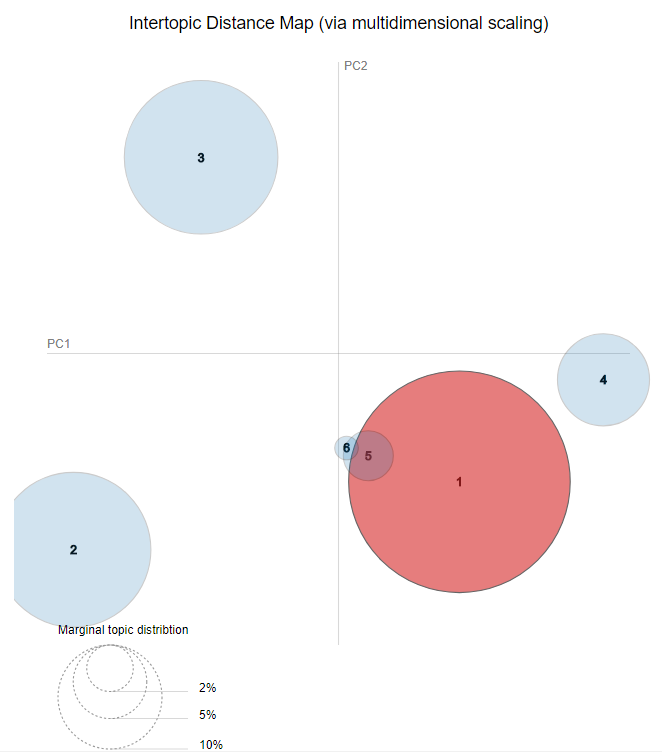
\includegraphics[width = 0.85 \textwidth]{img/lda/1.PNG}}
  \caption{Principal Component Analysis for Topic Modelling Digital Music Dataset}
\end{figure}

\begin{table}[h]
\centering
\begin{tabular}{ lllll }
% \toprule
%  &  &  &  &  \\
\midrule
music  & live  & like  & quot  & quot  \\
album  & james  & cd  & live  & mr  \\
soul   & time  & live  & jb  & brown  \\ 
like  & best  & just  & studio  & james  \\ 
great    & band  & band  & loose  & machine \\ 
right  & brown & bootsy  & world & band  \\ 
brown   & funk  & doing  &  time  &  sex \\ 
just   & album  & sex & great &  funk \\ 
\bottomrule          
\end{tabular}
\caption{Music Labels}
\label{Music Labels}
\end{table}



\begin{figure}[H]
  {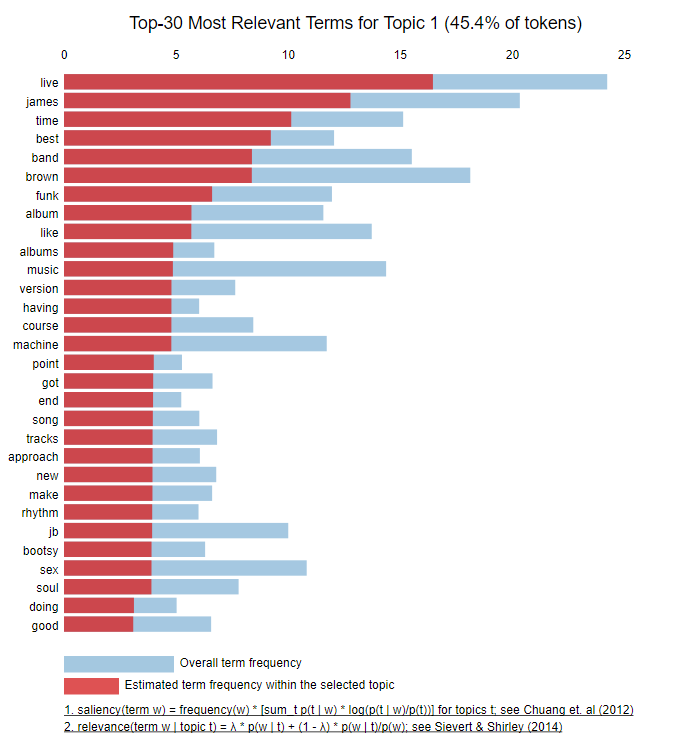
\includegraphics[width = 0.85 \textwidth]{img/lda/1a.PNG}}
  \caption{Topic Distribution on Digital Music Dataset}
\end{figure}


% \begin{table}[h]
% \centering
% \begin{tabular}{ lllll }
% \toprule
%  &  &  &  &  \\
% \midrule
% music  & live  & like  & quot  & quot  \\
% album  & james  & cd  & live  & mr  \\
% soul   & time  & live  & jb  & brown  \\ 
% like  & best  & just  & studio  & james  \\ 
% great    & band  & band  & loose  & machine \\ 
% right  & brown & bootsy  & world & band  \\ 
% brown   & funk  & doing  &  time  &  sex \\ 
% just   & album  & sex & great &  funk \\ 
% \bottomrule          
% \end{tabular}
% \caption{Labels Table}
% \label{Labels Table}
% \end{table}


\begin{figure}[H]
  {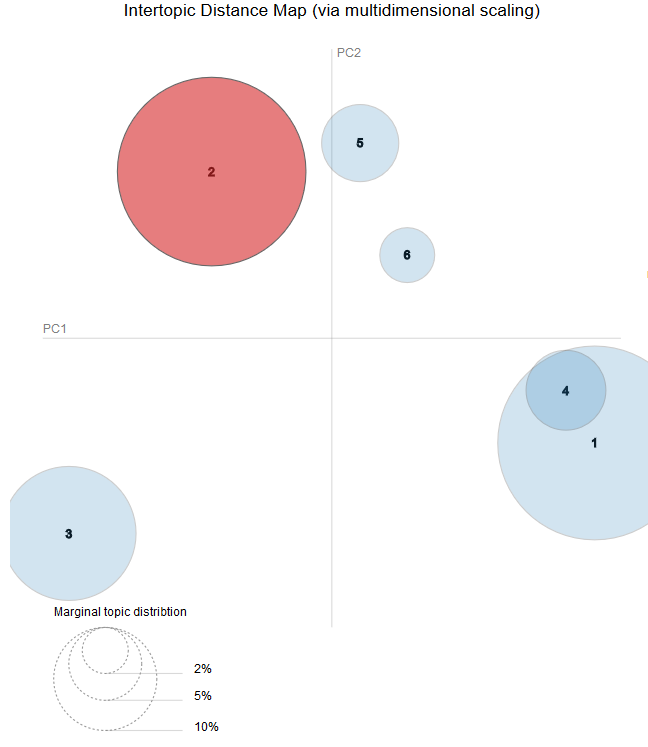
\includegraphics[width = 0.85 \textwidth]{img/lda/2.PNG}}
  \caption{Principal Component Analysis for Topic Modelling Health and Personal Care Dataset}
\end{figure}



\begin{table}[h]
\centering
\begin{tabular}{ llllll }
% \toprule
%   &  &  &  &  &  \\
\midrule
computer & fitbit & fitbit & day & walk & calories \\
calories & app & far & track & weight & fitbit \\
eat & sleep & lost & fitbit & just & active \\
burned & just & device & easy & device & app \\
weight & really & good & computer & read & steps \\
good & great & track & sleep & sleep & don \\
steps & need & read & great & help & burned \\
tells & does & kindle & like & stairs & help \\
\bottomrule          
\end{tabular}
\caption{Health and Personal Care Labels}
\label{Health and Personal Care Labels}
\end{table}

\begin{figure}[H]
  {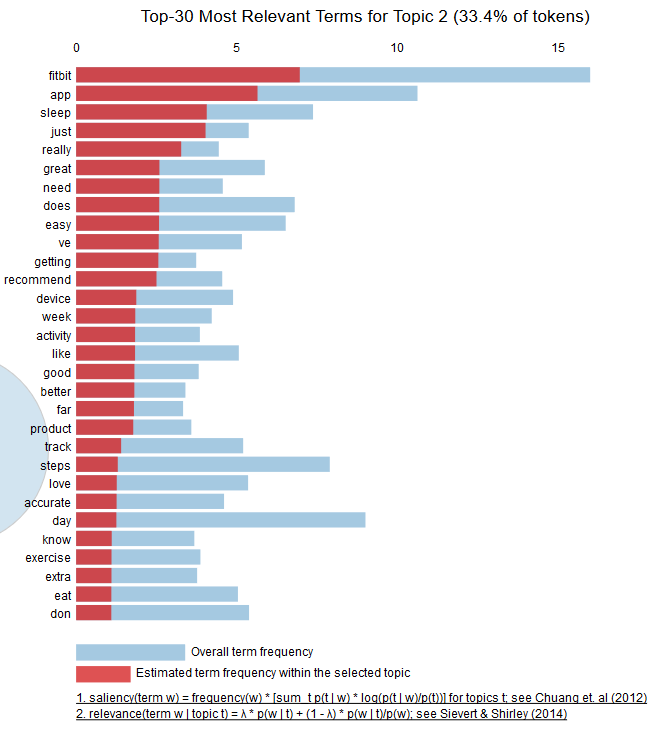
\includegraphics[width = 0.85 \textwidth]{img/lda/2a.PNG}}
  \caption{Topic Distribution on Health and Personal Care Dataset}
\end{figure}

\begin{figure}[H]
  {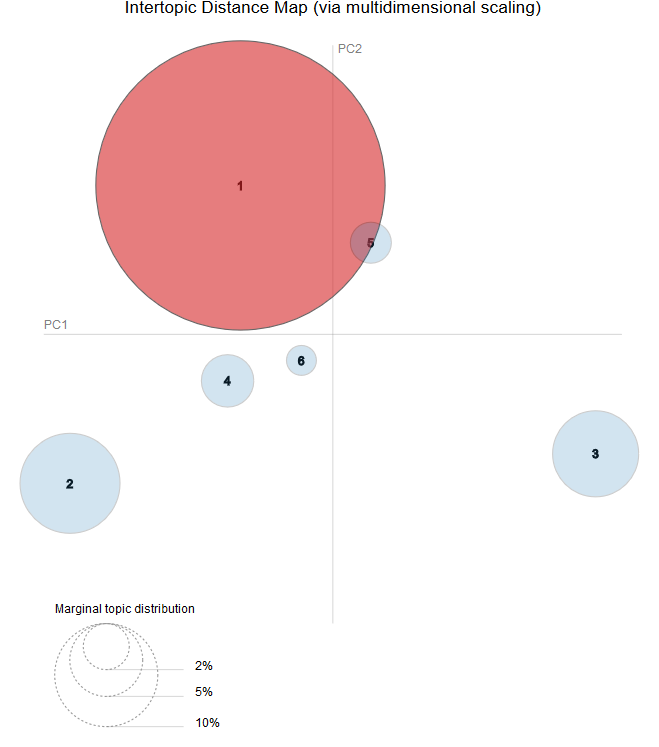
\includegraphics[width = 0.85 \textwidth]{img/lda/3.PNG}}
  \caption{Principal Component Analysis for Topic Modelling CellPhones and Accessories Dataset}
\end{figure}


\begin{table}[h]
\centering
\begin{tabular}{ lllll }
% \toprule
%  &  &  &  &  \\
\midrule
battery & batteries & red   & works  & quot  \\
charger & battery & charging & batteries  & mr  \\
charge & just   & blue  & charges     & brown  \\ 
phone & phone  &  charger  & product    & james  \\ 
batteries  & spare & use  & great   & machine \\ 
usb & brown & light & different  & band  \\ 
charging & like  &  works & charged  &  sex \\ 
use & port & sex & just &  thing  \\ 
\bottomrule          
\end{tabular}
\caption{Cell Phones and Accessories Labels}
\label{Cell Phones and Accessories Labels}
\end{table}

\begin{figure}[H]
  {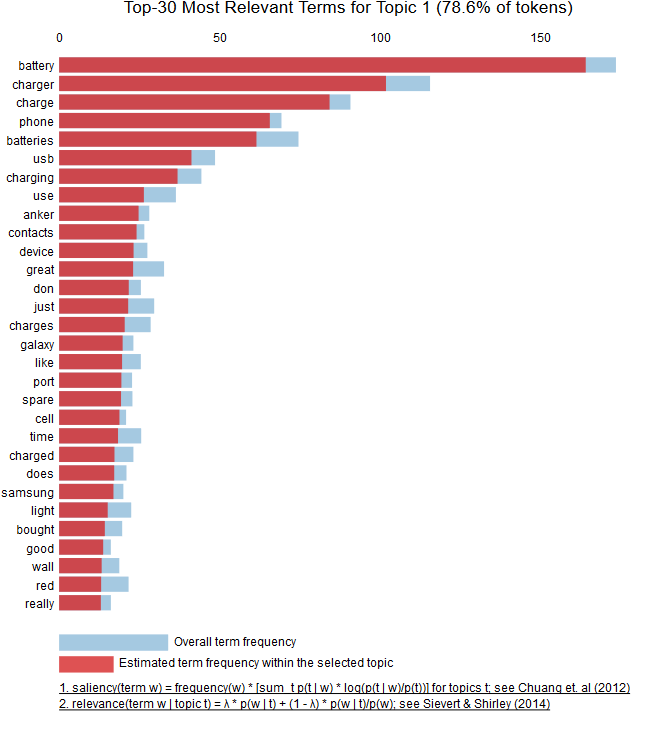
\includegraphics[width = 0.85 \textwidth]{img/lda/3a.PNG}}
  \caption{Topic Distribution on CellPhones and Accessories Dataset}
\end{figure}


This shows a significant increase in the model accuracy, consequently this type of approach can be used to improve the recommendations generated by the system.

\begin{itemize}
    \item Always recommend items based on gender. (Men and women always buy the same items as other men and women, respectively)
    \item Always recommend items based on age. (People at a certain age always buy same items as other people in the same age)
    \item Always recommend items based on domicile. (People from city X always buy the same items as other people from city X)
    \item Baselines have been used before any other extensive evaluation method, something that has been of great help when implementing the application, as these baselines can be seen as evaluation in its most basic form.
\end{itemize}




% \chapter{Discussion}
As stated in the introduction, this thesis aims to evaluate the performance
of Multi-Armed Bandit Algorithms in an e-commerce environment. In this
chapter evaluation of user-experience and comparisons with other algorithms
will be presented together with thoughts regarding the result and future work.

A
7.1

Evaluating The Result

The result can be evaluated depending on several different aspects. In this section focus
will be put on evaluation of performance and user-experience as well as some thoughts
regarding why the result turned out the way it did.

7.1.1

Performance

The percentage of correct predictions can be seen on the y-axis of the graphs in section
6.1. By comparing the graphs in figure 6.1 one can draw the conclusion that the best
recommendations are made in the time interval between one week to one month posterior to starting the application. Predictions in this period got an accuracy of 19 to 21
percent. Seeing how this is in a garment-based e-commerce environment it makes sense
that new collections of products are added every other month, whereas the products from
last month’s collection do not sell as good. The simulation made in these graphs starts
in late spring, 2012-05-01, meaning that recommendations of cloths for the summer are
more likely to be of satisfactory than a few months later when summer-based cloths are
recommended for the fall or winter. The conclusion here is that if this application was
to run in a live system, it would make sense to reset the trained data prior to releasing
a new collection and/or before each new season.
As mentioned earlier, the dataset used in this thesis contains only static data. Meaning
that for a prediction to be seen as correct, a recommended item has to be purchased at
38

7.1. EVALUATION

CHAPTER 7. DISCUSSION

some point in time after the recommendation is performed. The problem using static
data rather than testing an application live in this setting is that possibly good recommendations are not measured, because an item was not purchased. One can never know
if the user would have bought more products if products that she could possibly like
would be presented to her. Hence the only thing that can be measured is actual purchases, while in theory a user is likely to buy more products based on the recommended
items. Something that could be said to be certain about the application here is that it
predicts correct items with at least 19-21 percent accuracy and probably higher in most
cases.
All the graphs in Chapter 6 expressing anonymous data to some extent, proves that
taking a more privacy-preserving approach, actually gives worse performance in terms
of measuring successful recommendations. By comparing the graphs in figure 6.1 where
the algorithm is using all available context, with the other graphs in figure 6.2 where
the algorithm is using less context, it is possible to see a difference of about 6-10 percent
depending on which graphs are observed. It is hard to tell if it is worth it or not, but
seeing how things work in reality where most people accept any license agreement of applications or web-pages, one can draw the conclusion that as long as the observed data
is used in ways that benefit the actual user and not a third party, it is at least socially
acceptable. Facebook is a good example of this, which in their licence agreement [63]
state that they have all the rights to any data you submit or take part of online, when
using their services. They also state that your data will be accessible by companies and
third parties of their choosing.
There are also other aspects to a good result than through only measuring the number of
successful recommendations, such as user experience and satisfaction level of customers.
Unfortunately these are hard to measure without deploying the system live. See more
about user-experience under 7.1.2.
So far we have seen that the implemented application can predict shopping behaviour
of most users with a probability of around 20 percent. So the question is how well
does other similar applications perform on similar datasets. One similar application in
a similar setting can be seen in [61] where they use significantly different algorithms and
achieve correct recommendations with a probability of about 17 percent. The authors
of [61] make use of a collaborative filtering-based techniques, but with significantly better performance than the collaborative filtering-based algorithms used in this project.
Nevertheless, the content-based filtering implementation using Contextual Multi-Armed
Bandits in this thesis outperforms the algorithms used in [61], something that ought to
be considered as successful. In figure 7.1 below, the different implemented algorithms
of this thesis is presented with different colours, using the time interval of one month
because of its relevance as described above.

39

7.1. EVALUATION

CHAPTER 7. DISCUSSION

Predictions made of data from 1 month in time
25
Best Arm
All Arms
Popularity(Baseline)
Jaccard Similarity

Correct predictions (%)

20

15

10

5

0

0

2000

4000

6000

8000

10000

12000

14000

16000

Number of predictions

Figure 7.1: Graph showing the results of all implemented algorithms from one month in
time

And as can be seen in this graph, the Contextual Multi-Armed Bandit Algorithm outperforms all of the others. Notable is also that the popularity baseline algorithm appears
to have pretty high performance. Something that is easily realised why it is the case.
This strategy is very bad in other aspects as if taking User-Experience into account. See
section 7.1.2 for more details regarding this.
The next graph, in figure 7.2, shows the performance of all algorithms in different colours,
measuring performance of purchases over one year.

40

18000

7.1. EVALUATION

CHAPTER 7. DISCUSSION

Predictions made of data from 12 months in time
30
Best Arm
All Arms
Popularity(Baseline)
Jaccard Similarity

Correct predictions (%)

25

20

15

10

5

0

0

0.5

1

1.5

2

2.5

3

Number of predictions

3.5
×105

Figure 7.2: Graph showing the results of all implemented algorithms from one year in time

Here one can see that the result does not change even in the long run. All algorithms
perform best during the first months due to reasons expressed in the beginning of this
section, but even after a long time the order of good versus bad algorithms do not change.
Something notable is what happens in the time span between 1 and 3 months, where
we can see a dip in performance in terms of successful recommendations. The graph
stretches from 2012-05-01 to 2012-07-31. In this time period there is a shift in products
wanted by the users. A user that has bought for instance some pairs of jeans during
May has a high probability of being recommended jeans during the later months too.
However, during the summer it is more likely that the user wants to buy shorts and other
products more suitable for use during the summer. As can be seen in graph 7.2, the popularity curve also become worse during these months. This means that user-behaviour
is harder to predict during these months. This might be the case either because there is
a larger set of items that can be recommended, or because user behaviour is not as predictable during the summer as during the spring. As mentioned initially in this chapter,
it is also likely that new collections of garment are released before each season, which
might be another contributing factor to the dip in performance during the specific time
spans.
One could wonder: why did the collaborative filtering-based algorithm using Jaccard

41

7.1. EVALUATION

CHAPTER 7. DISCUSSION

Similarity perform so poorly with the Junkyard dataset, in comparison with the other
algorithms in this thesis and the ones described in [61]. This, of course, might depend on
a variety of different reasons such as algorithms or datasets being significantly different.
Seeing how the focus of this evaluation is on the performance of Multi-Armed Bandits,
further investigation of the poor result of the above mentioned will be left for future work.
As explained in 3.2, regret bounds are often used for measuring negative emotion experience in decision theory and probabilistic modelling. In figure 7.3 below, the total regret
is illustrated for ’All Arms’, ’Most Buys’ and ’Jaccard Similarity’ relative to the ’Best
Arm’.
Regret of All Arms, Popularity and Jaccard Similarity relative to the Best Arm

100

All Arms
Popularity(Baseline)
Jaccard Similarity

90

80

Regret (%)

70

60

50

40

30

20

10

0

2000

4000

6000

8000

10000

12000

14000

16000

Number of predictions

Figure 7.3: Regret of ’All Arms’, ’Most Buys’ and ’Jaccard Similarity’ relative to the Best
Arm.

An interesting scenario that was stumbled upon is if the following happens (7.4):

42

18000

7.1. EVALUATION

CHAPTER 7. DISCUSSION

Predictions made of data from 1 month in time
20
Best Arm
All Arms

18
16

Correct predictions (%)

14
12
10
8
6
4
2
0

0

1000

2000

3000

4000

5000

6000

Number of predictions

Figure 7.4: All Arms outperforming Best Arm for some time

What can be seen here is running the algorithm for six months, and where All Arms
seemingly perform better than the Best Arm at some point in time. There is a simple
explanation to this phenomenon. Posterior to running the algorithm, the algorithm looks
at all arms to see which one that is having the best performance. Thus the arm with
the best performance posterior to running the algorithm is not necessarily the best arm
throughout the whole simulation.

7.1.2

User-Experience

User-Experience is more tricky to measure than performance. Despite suggesting items
that are likely to be bought statistically, it does not mean that it will make a specific
customer happy. Recommending items that might be of no value for a specific customer,
but are best-sellers, is unarguably not the best way to present recommendations even
if it will show good performance. This can be seen in the graphs in figure 6.3 where
recommendations are made entirely based on whats the currently most bought items as
of the last week.

43

7000

7.1. EVALUATION

CHAPTER 7. DISCUSSION

Like a physical store
When visiting a physical store, you would not want the shopping assistant to only propose the same items as she is proposing to everyone else. For instance by proposing only
the best-sellers as of the last week, not taking anything else into consideration. Instead
you would want the shopping assistant to listen to what kind of items you like and have
enjoyed earlier, and what you are currently looking for. The same thing applies for most
people when browsing E-Commerce websites or platforms. If you browse for or buy certain items, the system should adapt to this and actually try to help you find what you
might be looking for in the future. That is if you are looking to buy a pair of shoes and
you are recommended ten different shirts, just because the shirts happened to be on sale
last week meaning that a lot of people have purchased them, you will not be satisfied or
any closer to finding the pair of shoes you were after.
If however, let us say, the shopping assistant was to follow you around noting what
you were looking at or even what you were buying in other stores, you would probably
find her creepy and probably stay away from her stores. This despite the fact that it
might mean ending up with an item you enjoy, faster. Once again, the same idea can
be applied in E-Commerce systems; using all data you can from a specific user is not
ethically acceptable. It is however more socially acceptable as described in 7.1.1. This
could be data such as cookie-based history of other browsed web sites. It could also be
data retrieved from buying and selling information gathered in other systems.
Our implementation
When implementing the algorithm in this project, the physical store was kept in mind.
Users should not relate to the system as the creepy shopping assistant. The implemented
application thus only focus on using data gathered from the platform which it was built
for and even there discussing different privacy-preserving aspects. Neither should users
relate to the system as the lazy shopping assistant who only gives the same recommendations to everyone. Instead focus was put on making the customers feel that the system or
shopping assistant actually proposed valid items that the customer could be interested
in. This by giving ten recommendations that match the specific customer’s profile.
Taking it live
Observing the shopping history of a user in the store is an intuitively good technique to
figure out what the user is interested in. However, if taking the system live,predictions
would also based on the current live session. The taste of a user would probably most
often be similar from the different times she visits the website, but she might want to
shop from different categories during different sessions. Looking for shoes at one time
should not mean that the user only gets shoe recommendations the second time she
browses the site. If the user however only looks for gender-specific items, most of the
time there would be no point in suggesting the opposite.

44

7.2. FUTURE WORK

CHAPTER 7. DISCUSSION

Best-seller recommendations are not useless in any way. Using this application in a
live setting could mean using best-seller recommendations on the front page so that
people occasionally browsing the page in hopes of finding something they like might get
lucky, while the personalised recommendations could be used on the specific user-pages.

7.2

Future Work

There are still issues related with the result of this project that could be desirable to
address, but that goes out of the scope of this thesis. In this section we will present
some concrete ideas of possible future work related to this thesis.

7.2.1

Synthetic Data

Synthetic data is, as opposed to authentic data, generated within some behavioural
model. It is explained in [64] and described as: ”Synthetic data can be defined as data
that are generated by simulated users in a simulated system, performing simulated actions.
One obvious use-area for synthetic data is the possibility of doing realistic testing of
a system or parts of a system before deploying them live. There are however many difficulties that need to be considered before implementation can start. Difficulties that are
not entirely addressed in current research as it varies in different settings and systems.

7.2.2

Extensive Collaborative Filtering-Based Algorithm

The implemented collaborative filtering-based algorithm in this thesis perform poorly in
comparison to what current research expresses when describing collaborative filteringbased algorithms. It would be interesting to make use of different similarity computing
techniques to see if it could, first of all, provide a better result than the implemented
collaborative filtering-based algorithm in this thesis, but also if it could beat the performance of the Contextual Multi-Armed Bandit Algorithm implemented in this thesis.

45

8
Conclusion
n this thesis the performance of Contextual Multi-Armed Bandit Algorithms have
been measured and evaluated in terms of successful recommendations, user-experience
and possibility of working using privacy-preserving methods, in a garment-based
e-commerce environment. The result can be seen in chapter 6. In the aspect of making successful recommendations and giving a good user-experience the results look good.
But also in the cases where privacy-preserving approaches have been taken, the results
are fairly good. Depending on the setting and system, if required, it would thereby be
feasible to consider even the privacy-preserving modes of the algorithm as performance
in terms of successful recommendations are fairly good despite those restrictions.

I

8.1

The Research Question

In the introduction we defined the research question as:
Would the algorithmic approach of Contextual Multi-Armed Bandit Algorithms perform
well enough to belong among the different algorithmic approaches to consider when implementing recommender systems?
A justified answer to this question, with respect to the results presented in Chapter 6 and
the reasoning of the results presented in Chapter 7, is ”yes”. A reasonable conclusion that
can be made from observing the result where purchasing behaviour is predicted with a
probability of over 20 % is that considering Contextual Multi-Armed Bandit Algorithms
when implementing recommender systems is highly appropriate.
The more complex but also most suitable answer to the research question is ”probably”
or ”it depends on the setting and environment”. As the name Contextual Multi-Armed
Bandit Algorithms indicates, the algorithm makes use of contexts such as a user’s context, personal information, and might thus not be eligible in systems where all data is to
be totally anonymous or where only non-personal data exists. However, as can be seen



\chapter{Conclusion and Future Work}

The results obtained by applying both Probablistic Matrix Factorization and the Latent Dirichlet Allocation are very satifying and also explained most of the recomendations. The results are very superior as compared to other algorithms applied on the same datasets by Amazon. 

In future, we will be pleased to have more work in the stochastic machine learning algorithms applied to Recommendation Systems. More algorithms with much scope must be tested to provide the better clarity in this text review domain.





\clearpage

\nocite{*}

\bibliography{final_thesis}
%% special package for bibliography
%\bibliographystyle{plainnat}
%\bibliographystyle{plain}
%\bibliographystyle{unsrt}
\bibliographystyle{apalike}
% \printbibliography

\end{document}

